\documentclass[10pt]{article}
\usepackage[polish]{babel}
\usepackage[utf8]{inputenc}
\usepackage[T1]{fontenc}
\usepackage{amsmath}
\usepackage{amsfonts}
\usepackage{amssymb}
\usepackage[version=4]{mhchem}
\usepackage{stmaryrd}
\usepackage{graphicx}
\usepackage[export]{adjustbox}
\graphicspath{ {./images/} }

\title{LIGA MATEMATYCZNA \\
 FINAE \\
 30 marca 2011 \\
 SZKOŁA PONADGIMNAZJALNA }

\author{}
\date{}


\begin{document}
\maketitle
\section*{ZADANIE 1.}
Na okręgu napisano jedenaście liczb. Suma każdych trzech kolejnych jest taka sama. Jedną z liczb jest 9. Wyznacz pozostałe liczby.

\section*{ZADANIE 2.}
Rozwiąż układ równań

\[
\left\{\begin{array}{l}
a b=a+b+1 \\
b c=b+c+2 \\
a c=a+c+5
\end{array}\right.
\]

\section*{ZADANIE 3.}
Wykaż, że dla dowolnych liczb całkowitych \(a\) i \(b\) liczba \(a^{3} b-a b^{3}\) jest podzielna przez 3.

\section*{ZADANIE 4.}
Dany jest pięciokąt wypukły \(A B C D E\), w którym przekątna \(B D\) jest równoległa do boku \(A E\), a przekątna \(C E\) jest równoległa do boku \(A B\). Wykazać, że pola trójkątów \(A B C\) i \(A D E\) są równe.

\section*{ZADANIE 5.}
Wykaż, że kwadrat liczby pierwszej większej od 3 z dzielenia przez 12 daje resztę 1.

\section*{ZADANIE 6.}
Rozwiąż równanie \(x^{2}+4 x-y^{2}-2 y-8=0 \mathrm{w}\) zbiorze liczb naturalnych.

\section*{ZADANIE 7.}
Czworokąt \(A B C D\) jest kwadratem. Punkty \(E\) i \(F\) leżą na bokach \(B C\) i \(C D\) tego kwadratu tak, że \(\measuredangle E A F=45^{\circ}\). Wykaż, że \(|B E|+|D F|=|E F|\).\\
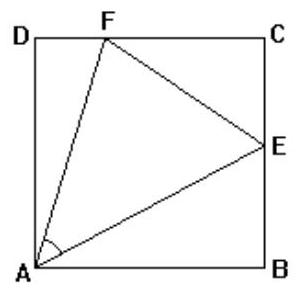
\includegraphics[max width=\textwidth, center]{2024_11_21_cdfba54282833f1a9b44g-1}


\end{document}